\chapter{Implementação da Solução}
\label{sec:4-Implementacao}

Este capítulo aprofunda o processo de desenvolvimento da solução para o problema do projeto em 
análise de acordo com a análise e os princípios de \textit{design} discutidos no capítulo anterior. 
Além disso, é efetuada uma análise cuidada dos resultados obtidos através das decisões anteriores, 
revelando os resultados consequentes e a sua concordância com os objetivos discutidos anteriormente.

\section{Tecnologias Utilizadas}

Durante o desenvolvimento do projeto, foram utilizadas várias tecnologias e ferramentas para a 
implementação da solução. Entre as mais relevantes, destacam-se:

\begin{itemize}
  \item \textbf{Apache Storm \cite{storm}:} \textit{Framework} de processamento de 
    \textit{streaming} em tempo real;
  \item \textbf{Apache Kafka \cite{kafka}:} Plataforma de mensagens distribuída;
  \item \textbf{Apache Zookeeper \cite{zookeeper}:} Serviço de coordenação distribuída;
  \item \textbf{Grafana \cite{grafana}:} Plataforma de análise e visualização de dados;
  \item \textbf{Jenkins \cite{jenkins}:} Servidor de automação de \textit{builds}; 
  \item \textbf{Nimbus \cite{nimbus}:} Servidor centralizado que coordena e distribui as topologias 
    do \textit{Apache Storm};
  \item \textbf{Splunk \cite{splunk}:} Plataforma de análise de eventos e dados;
\end{itemize}

\section{Descrição da implementação}

De forma a conseguir atingir os objetivos pretendidos, analisados no capítulo anterior, é
necessário ter em conta vários processos que fazem parte da implementação da solução. Para 
facilitar a compressão e análise dos mesmos vão ser apresentados os vários passos e algum 
suporte, como diagramas, que ajudam a ter uma melhor compreensão de todo o processo necessário
para atingir estes objetivos.

\subsection{Scaledown do Cluster}

Um dos processos necessários para conseguir atingir a solução pretendida é efetuar a alteração
de configurações do uso de recursos (\gls{flavour}) dos \glspl{cluster} existentes. Como
referido anteriormente todos os processos de infraestrutura são geridos internamente pela Blip e,
desta forma, têm os seus processos próprios para este tipo de operações.

Neste caso, as configurações dos recursos dos serviços é efetuado a partir de um repositório 
de configurações específicas de infraestrutura para cada um dos serviços. Ao efetuar uma alteração
neste repositório é automaticamente despoletado um Job Jenkins que trata da criação do artefacto
da nova versão e executa a \textit{pipeline} correspondente no ambiente de \ac{QA}.

Todo este processo é automatizado e, por isso, é necessário compreender quais são os mecanismos
existentes de forma a trabalhar de forma eficiente com os mesmos. A Figura \ref{scaledown-nxt} 
ilustra o processo de \textit{scaledown} de um \textit{cluster} no ambiente de NXT e qual o 
procedimento adicional em caso de necessidade de reversão da operação.

\begin{figure}[H]
  \centerline{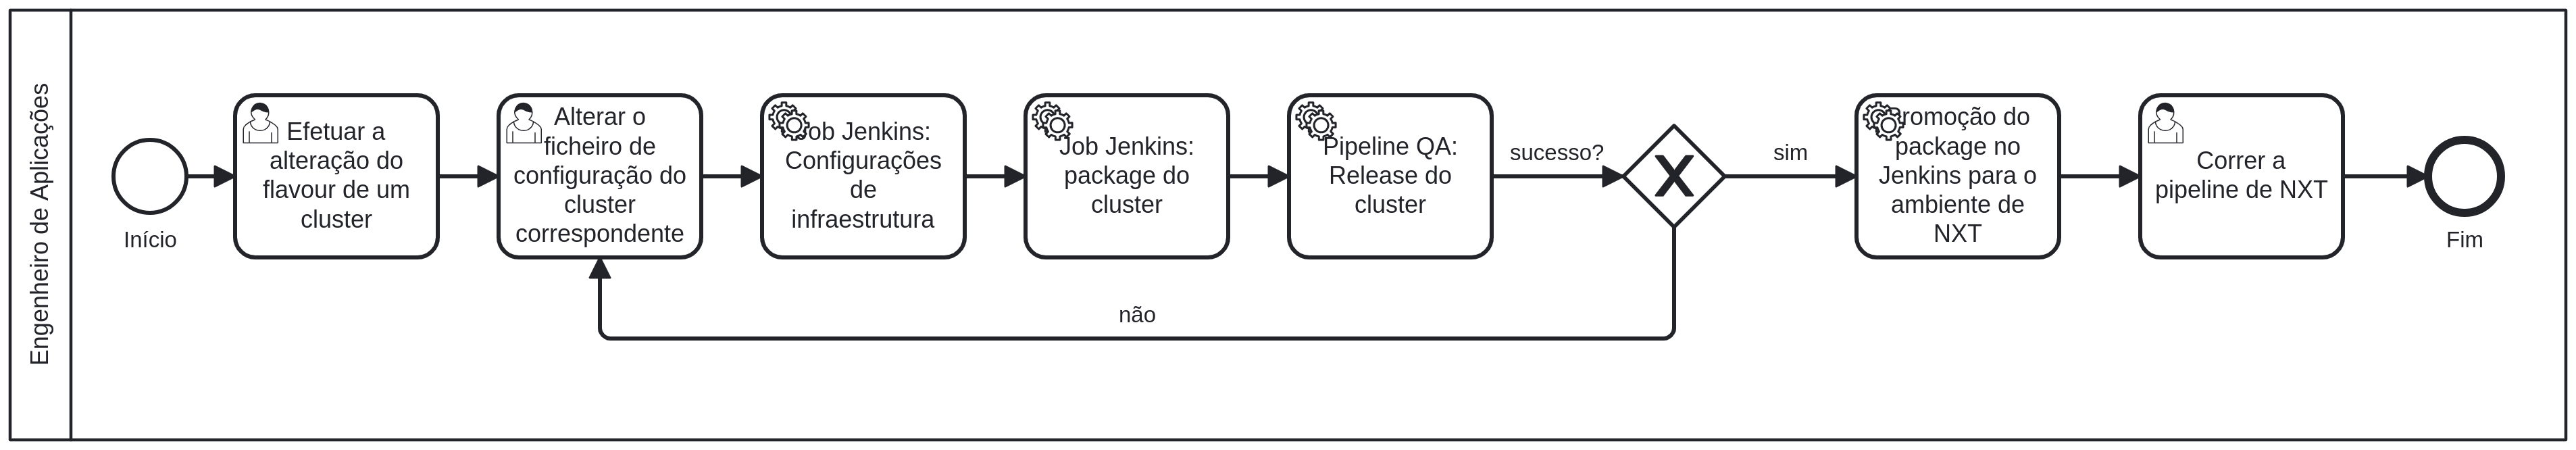
\includegraphics[scale=0.12]{media/content/impl/scaledown_nxt.png}}
  \caption{Processo de \textit{scaledown} de um \textit{cluster} no ambiente de NXT}
  \label{scaledown-nxt}
\end{figure}

\todo[inline]{Incluir BPMNs do processo de criação de novos clusters (simplificado}

\section{Testes}

\todo[inline]{TODO}

\section{Avaliação da Solução}

\todo[inline]{TODO}

